\chapter{Технологическая часть}

В данном разделе будут описаны средства реализации, будет представлена диаграмма классов, а так же интерфейс ПО. Так же будут представлены реализации алгоритмов, выбранных ранее.

\section{Средства реализации. Диаграмма классов}
Для реализации программного обеспечения был выбран язык C\# по следующим причинам:
\begin{enumerate}
	\item Он поддерживает объектно-ориентированный стиль программирования;
	\item Личный опыт разработки на данном языке позволяет эффективно решать поставленные задачи;
	\item Язык обладает высокой производительностью, что важно при трассировке лучей и выполнении вычислений на процессоре.
\end{enumerate}

В качестве среды разработки была выбрана Visual Studio \cite{b7}, поскольку она достаточно удобна и обладает всем необходимым функционалом для реализации поставленной задачи. В частности, использование библиотеки WPF \cite{b6} позволяет реализовать современный и функциональный пользовательский интерфейс, а фреймворк .NET 8.0 \cite{b8} предоставляет платформу для создания высокопроизводительных кроссплатформенных приложений.

На рисунке ниже представлена UML-диаграмма классов, необходимых для решения поставленной задачи. Она отображает структуру и взаимосвязи между  классами, что позволяет наглядно представить архитектуру программного обеспечения и взаимодействие его компонентов.

\begin{table}[H]
	\centering
	\begin{tabular}{p{1\linewidth}}
		\centering
		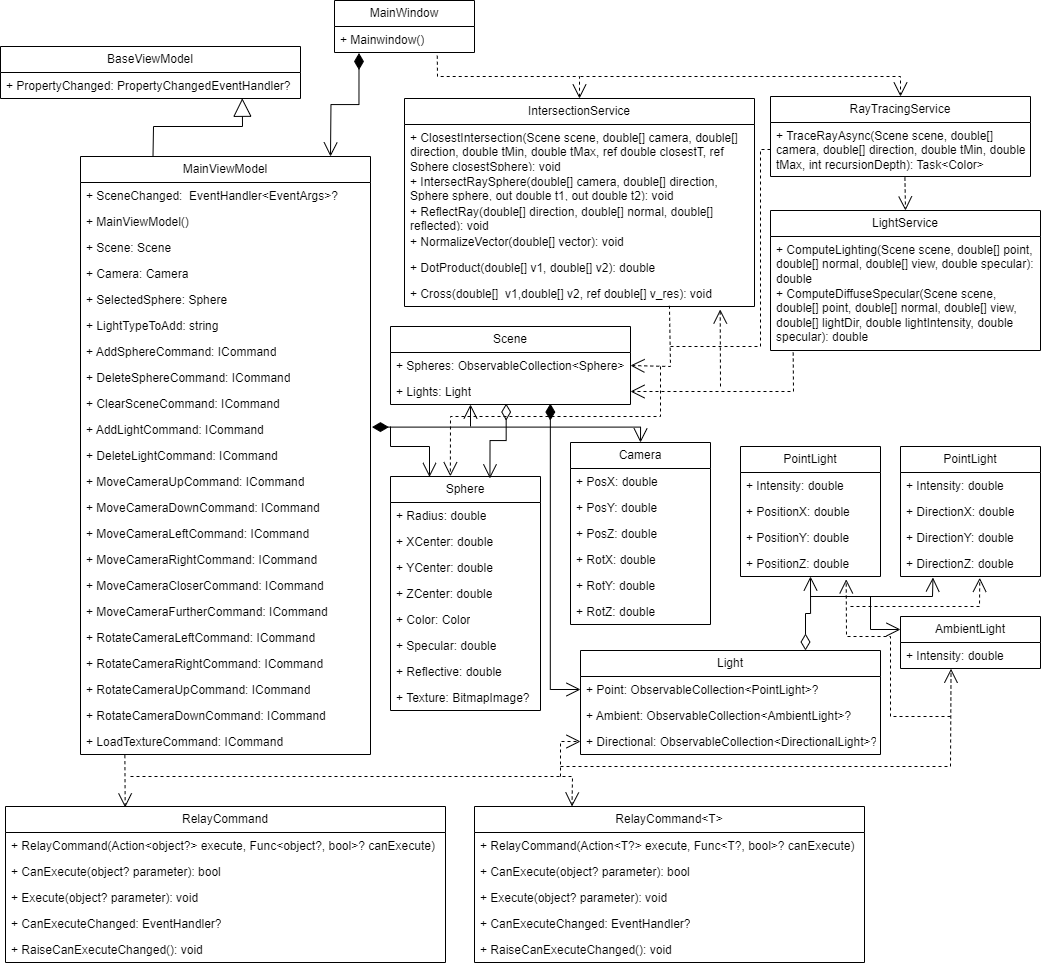
\includegraphics[width=0.9\linewidth]{include/3-1.drawio.png}
		\captionof{figure}{UML-диаграмма классов реализуемого ПО}
		\label{img:3-1}
	\end{tabular}
\end{table}

\section{Реализация алгоритмов}

Ниже представлен класс, реализующий логику пускания лучей и их пересечения с объектами.
\begin{lstlisting}[caption={Класс IntersectionService}, label={lst:3-2}]
public static class IntersectionService
{
	public static void ClosestIntersection(Scene scene, Vector3 camera, Vector3 direction, double tMin, double tMax, out double closestT, out Sphere? closestSphere)
	{
		closestT = double.PositiveInfinity;
		closestSphere = null;
		
		foreach (var sphere in scene.Spheres)
		{
			IntersectRaySphere(camera, direction, sphere, out double t1, out double t2);
			
			if (tMin <= t1 && t1 <= tMax && t1 < closestT)
			{
				closestT = t1;
				closestSphere = sphere;
			}
			
			if (tMin <= t2 && t2 <= tMax && t2 < closestT)
			{
				closestT = t2;
				closestSphere = sphere;
			}
		}
	}
	
	private static void IntersectRaySphere(Vector3 camera, Vector3 direction, Sphere sphere, out double t1, out double t2)
	{
		Vector3 oc = camera - sphere.Center;
		double a = Vector3.DotProduct(direction, direction);
		double b = 2.0 * Vector3.DotProduct(oc, direction);
		double c = Vector3.DotProduct(oc, oc) - sphere.Radius * sphere.Radius;
		double discriminant = b * b - 4 * a * c;
		
		if (discriminant < 0)
		{
			t1 = t2 = double.PositiveInfinity;
		}
		else
		{
			double sqrtDiscriminant = Math.Sqrt(discriminant);
			t1 = (-b - sqrtDiscriminant) / (2.0 * a);
			t2 = (-b + sqrtDiscriminant) / (2.0 * a);
		}
	}
	
	public static Vector3 ReflectRay(Vector3 direction, Vector3 normal)
	{
		double dotProduct = Vector3.DotProduct(direction, normal);
		return  normal * (2 * dotProduct) - direction;
	}
}
\end{lstlisting}

Класс, отвечающий за внедрение света:
\begin{lstlisting}[caption={Класс LightService}, label={lst:3-3}]
public static class LightService
{
	public static double ComputeLighting(Scene scene, Vector3 point, Vector3 normal, Vector3 view, double specular)
	{
		double intensity = 0;
		
		foreach (var ambient in scene.Lights.AmbientLights)
		intensity += ambient.Intensity;
		
		foreach (var pointLight in scene.Lights.PointLights)
		{
			Vector3 lightDir = pointLight.Position - point;
			lightDir.Normalize();
			intensity += ComputeDiffuseSpecular(point, normal, view, lightDir, pointLight.Intensity, specular);
		}
		
		foreach (var directional in scene.Lights.DirectionalLights)
		{
			Vector3 lightDir = new Vector3(directional.Direction.X, directional.Direction.Y, directional.Direction.Z);
			lightDir.Normalize();
			intensity += ComputeDiffuseSpecular(point, normal, view, lightDir, directional.Intensity, specular);
		}
		
		return intensity;
	}
	
	private static double ComputeDiffuseSpecular(Vector3 point, Vector3 normal, Vector3 view, Vector3 lightDir, double lightIntensity, double specular)
	{
		double diffuseIntensity = Vector3.DotProduct(normal, lightDir) * lightIntensity;
		diffuseIntensity = Math.Max(diffuseIntensity, 0);
		
		double specularIntensity = 0;
		if (specular >= 0)
		{
			Vector3 reflectDir = IntersectionService. ReflectRay(lightDir, normal);
			double spec = Vector3.DotProduct(reflectDir, view);
			if (spec > 0)
			{
				specularIntensity = Math.Pow(spec, specular) * lightIntensity;
			}
		}
		
		return Math.Max(0, Math.Min(1, diffuseIntensity + specularIntensity));
	}
}
\end{lstlisting}

Класс который отвечает за трассировку. Он так же выполняет учет текстуры, поскольку при трассировке вычисляются нормали и удобно сразу же вносить в них возмущения.

\begin{lstlisting}[caption={Класс RayTracingService}, label={lst:3-5}]
public static class RayTracingService
{
	public static async Task<Color> TraceRayAsync(Scene scene, Vector3 camera, Vector3 direction, double tMin, double tMax, int recursionDepth)
	{
		IntersectionService.ClosestIntersection(scene, camera, direction, tMin, tMax, out double closestT, out Sphere? closestSphere);
		
		if (closestSphere == null)
		{
			return Colors.LightBlue;
		}
		
		Vector3 intersectionPoint = camera + direction * closestT;
		Vector3 normal = intersectionPoint - closestSphere.Center;
		normal.Normalize();
		
		if (closestSphere.Texture != null)
		{
			
			switch (closestSphere.TextureType)
			{
				case TextureType.HeightMap:
				normal = AdjustNormalWithHeightMap(closestSphere.Texture, normal, intersectionPoint);
				break;
				case TextureType.NormalMap:
				Color textureColor = await GetColorFromTextureAsync(closestSphere, normal);
				normal = AdjustNormalWithNormalMap(closestSphere.Texture, normal, textureColor);
				break;
				case TextureType.ParallaxMap:
				normal = AdjustNormalWithParallaxMap(closestSphere.Texture, normal, intersectionPoint);
				break;
			}
			normal.Normalize();
		}
		
		Vector3 viewDirection = -direction;
		double intensity = LightService.ComputeLighting(scene, intersectionPoint, normal, viewDirection, closestSphere.Specular);
		Color localColor = AdjustIntensity(closestSphere.Color, intensity);
		
		double reflectivity = closestSphere.Reflective;
		if (recursionDepth <= 0 || reflectivity <= 0)
		{
			return localColor;
		}
		
		Vector3 reflectionDirection = IntersectionService.ReflectRay(viewDirection, normal);
		Color reflectionColor = await TraceRayAsync(scene, intersectionPoint, reflectionDirection, 0.001, double.PositiveInfinity, recursionDepth - 1);
		Color finalColor = AdjustReflection(localColor, reflectionColor, reflectivity);
		
		return finalColor;
	}
	
	private static Color AdjustIntensity(Color color, double intensity)
	{
		byte r = (byte)Math.Min(255, Math.Max(0, color.R * intensity));
		byte g = (byte)Math.Min(255, Math.Max(0, color.G * intensity));
		byte b = (byte)Math.Min(255, Math.Max(0, color.B * intensity));
		return Color.FromRgb(r, g, b);
	}
	
	private static Color AdjustReflection(Color localColor, Color reflectionColor, double reflectivity)
	{
		byte r = (byte)Math.Min(255, Math.Max(0, localColor.R * (1 - reflectivity) + reflectionColor.R * reflectivity));
		byte g = (byte)Math.Min(255, Math.Max(0, localColor.G * (1 - reflectivity) + reflectionColor.G * reflectivity));
		byte b = (byte)Math.Min(255, Math.Max(0, localColor.B * (1 - reflectivity) + reflectionColor.B * reflectivity));
		return Color.FromRgb(r, g, b);
	}
	
	private static async Task<Color> GetColorFromTextureAsync(Sphere sphere, Vector3 normal)
	{
		double u = 0;
		double v = 0;
		
		ComputeTextureCoordinates(normal, ref u, ref v);
		
		int x = (int)(u * sphere.Texture?.PixelWidth ?? 0);
		int y = (int)(v * sphere.Texture?.PixelHeight ?? 0);
		
		var pixels = new byte[4];
		
		await Application.Current.Dispatcher.InvokeAsync(() =>
		{
			sphere.Texture?.CopyPixels(new Int32Rect(x, y, 1, 1), pixels, 4, 0);
		});
		
		return Color.FromArgb(pixels[3], pixels[2], pixels[1], pixels[0]);
	}
	
	private static void ComputeTextureCoordinates(Vector3 normal, ref double u, ref double v)
	{
		double phi = Math.Atan2(normal.Y, normal.X);
		double theta = Math.Acos(normal.Z);
		
		u = (phi + Math.PI) / (2.0 * Math.PI);
		v = theta / Math.PI;
	}
	
	private static Vector3 AdjustNormalWithHeightMap(BitmapSource heightMap, Vector3 normal, Vector3 intersectionPoint, double heightMapIntensity = 10.0)
	{
		double u = 0;
		double v = 0;
		ComputeTextureCoordinates(normal, ref u, ref v);
		
		int width = heightMap.PixelWidth;
		int height = heightMap.PixelHeight;
		
		int x = (int)(u * width);
		int y = (int)(v * height);
		
		x = Math.Max(0, Math.Min(width - 1, x));
		y = Math.Max(0, Math.Min(height - 1, y));
		
		byte[] currentPixel = new byte[4];
		heightMap.CopyPixels(new Int32Rect(x, y, 1, 1), currentPixel, 4, 0);
		
		double h = currentPixel[0] / 255.0;
		
		Vector3 gradient = new Vector3(0, 0, 1.0);
		
		if (x > 0 && x < width - 1)
		{
			byte[] leftPixel = new byte[4];
			byte[] rightPixel = new byte[4];
			
			heightMap.CopyPixels(new Int32Rect(x - 1, y, 1, 1), leftPixel, 4, 0);
			heightMap.CopyPixels(new Int32Rect(x + 1, y, 1, 1), rightPixel, 4, 0);
			
			double hLeft = leftPixel[0] / 255.0;
			double hRight = rightPixel[0] / 255.0;
			
			gradient.X = (hRight - hLeft) * heightMapIntensity;
		}
		
		if (y > 0 && y < height - 1)
		{
			byte[] topPixel = new byte[4];
			byte[] bottomPixel = new byte[4];
			
			heightMap.CopyPixels(new Int32Rect(x, y - 1, 1, 1), topPixel, 4, 0);
			heightMap.CopyPixels(new Int32Rect(x, y + 1, 1, 1), bottomPixel, 4, 0);
			
			double hTop = topPixel[0] / 255.0;
			double hBottom = bottomPixel[0] / 255.0;
			
			gradient.Y = (hBottom - hTop) * heightMapIntensity;
		}
		
		Vector3 perturbedNormal = normal + new Vector3(-gradient.X, -gradient.Y, 1.0);
		perturbedNormal.Normalize();
		
		return perturbedNormal;
	}
	
	
	private static Vector3 AdjustNormalWithNormalMap(BitmapSource texture, Vector3 normal, Color textureColor, double normalMapIntensity = 0.45)
	{
		double x = ((textureColor.R) / 255.0) * 2.0 - 1.0;
		double y = ((textureColor.G) / 255.0) * 2.0 - 1.0;
		
		double z = Math.Sqrt(Math.Max(0.0, 1.0 - Math.Clamp(x * x + y * y, 0.0, 1.0)));
		
		Vector3 normalMapNormal = new Vector3(x, y, z);
		normalMapNormal.Normalize();
		
		return Vector3.Lerp(normal, normalMapNormal, normalMapIntensity);
	}
	
	
	private static Vector3 AdjustNormalWithParallaxMap(BitmapSource parallaxMap, Vector3 normal, Vector3 viewDirection, double heightMapIntensity = 10.0)
	{
		double u = 0;
		double v = 0;
		ComputeTextureCoordinates(normal, ref u, ref v);
		
		int width = parallaxMap.PixelWidth;
		int height = parallaxMap.PixelHeight;
		
		int x = (int)(u * width) % width;
		int y = (int)(v * height) % height;
		
		x = (x + width) % width;
		y = (y + height) % height;
		
		byte[] currentPixel = new byte[4];
		parallaxMap.CopyPixels(new Int32Rect(x, y, 1, 1), currentPixel, 4, 0);
		double heightValue = currentPixel[0] / 255.0;
		
		Vector3 viewDirXY = new Vector3(viewDirection.X, viewDirection.Y, 0);
		viewDirXY.Normalize();
		
		double parallaxScale = 0.05;
		
		Vector3 parallaxOffset = viewDirXY * (heightValue * heightMapIntensity * parallaxScale);
		
		parallaxOffset.X = (parallaxOffset.X + width) % width;
		parallaxOffset.Y = (parallaxOffset.Y + height) % height;
		
		double uAdj = (u - parallaxOffset.X / width + 1.0) % 1.0;
		double vAdj = (v - parallaxOffset.Y / height + 1.0) % 1.0;
		
		int adjX = (int)(uAdj * width) % width;
		int adjY = (int)(vAdj * height) % height;
		
		adjX = (adjX + width) % width;
		adjY = (adjY + height) % height;
		
		byte[] adjustedPixel = new byte[4];
		parallaxMap.CopyPixels(new Int32Rect(adjX, adjY, 1, 1), adjustedPixel, 4, 0);
		
		double hX = 0.0;
		double hY = 0.0;
		
		if (adjX > 0 && adjX < width - 1)
		{
			byte[] leftPixel = new byte[4];
			byte[] rightPixel = new byte[4];
			
			parallaxMap.CopyPixels(new Int32Rect((adjX - 1 + width) % width, adjY, 1, 1), leftPixel, 4, 0);
			parallaxMap.CopyPixels(new Int32Rect((adjX + 1) % width, adjY, 1, 1), rightPixel, 4, 0);
			
			double hLeft = leftPixel[0] / 255.0;
			double hRight = rightPixel[0] / 255.0;
			
			hX = (hRight - hLeft) * heightMapIntensity;
		}
		
		if (adjY > 0 && adjY < height - 1)
		{
			byte[] topPixel = new byte[4];
			byte[] bottomPixel = new byte[4];
			
			parallaxMap.CopyPixels(new Int32Rect(adjX, (adjY - 1 + height) % height, 1, 1), topPixel, 4, 0);
			parallaxMap.CopyPixels(new Int32Rect(adjX, (adjY + 1) % height, 1, 1), bottomPixel, 4, 0);
			
			double hTop = topPixel[0] / 255.0;
			double hBottom = bottomPixel[0] / 255.0;
			
			hY = (hBottom - hTop) * heightMapIntensity;
		}
		
		Vector3 perturbedNormal = new Vector3(-hX, -hY, 1.0);
		perturbedNormal.Normalize();
		
		return normal + perturbedNormal;
	}
}
\end{lstlisting}

Для ускорения работы программы методы трассировки были реализованы асинхронными, поскольку алгоритм позволяет производить вычисления для каждого из лучей не зависимо от предыдущих и последующих результатов. Это очень сильно ускоряет работу программы и позволяет сделать интерфейс более отзывчивым, а работу в программе более приятной для пользователя.

\section{Интерфейс программного обеспечения}

На рисунке \ref{img:3-2} представлен интерфейс программы.

\begin{table}[H]
	\centering
	\begin{tabular}{p{1\linewidth}}
		\centering
		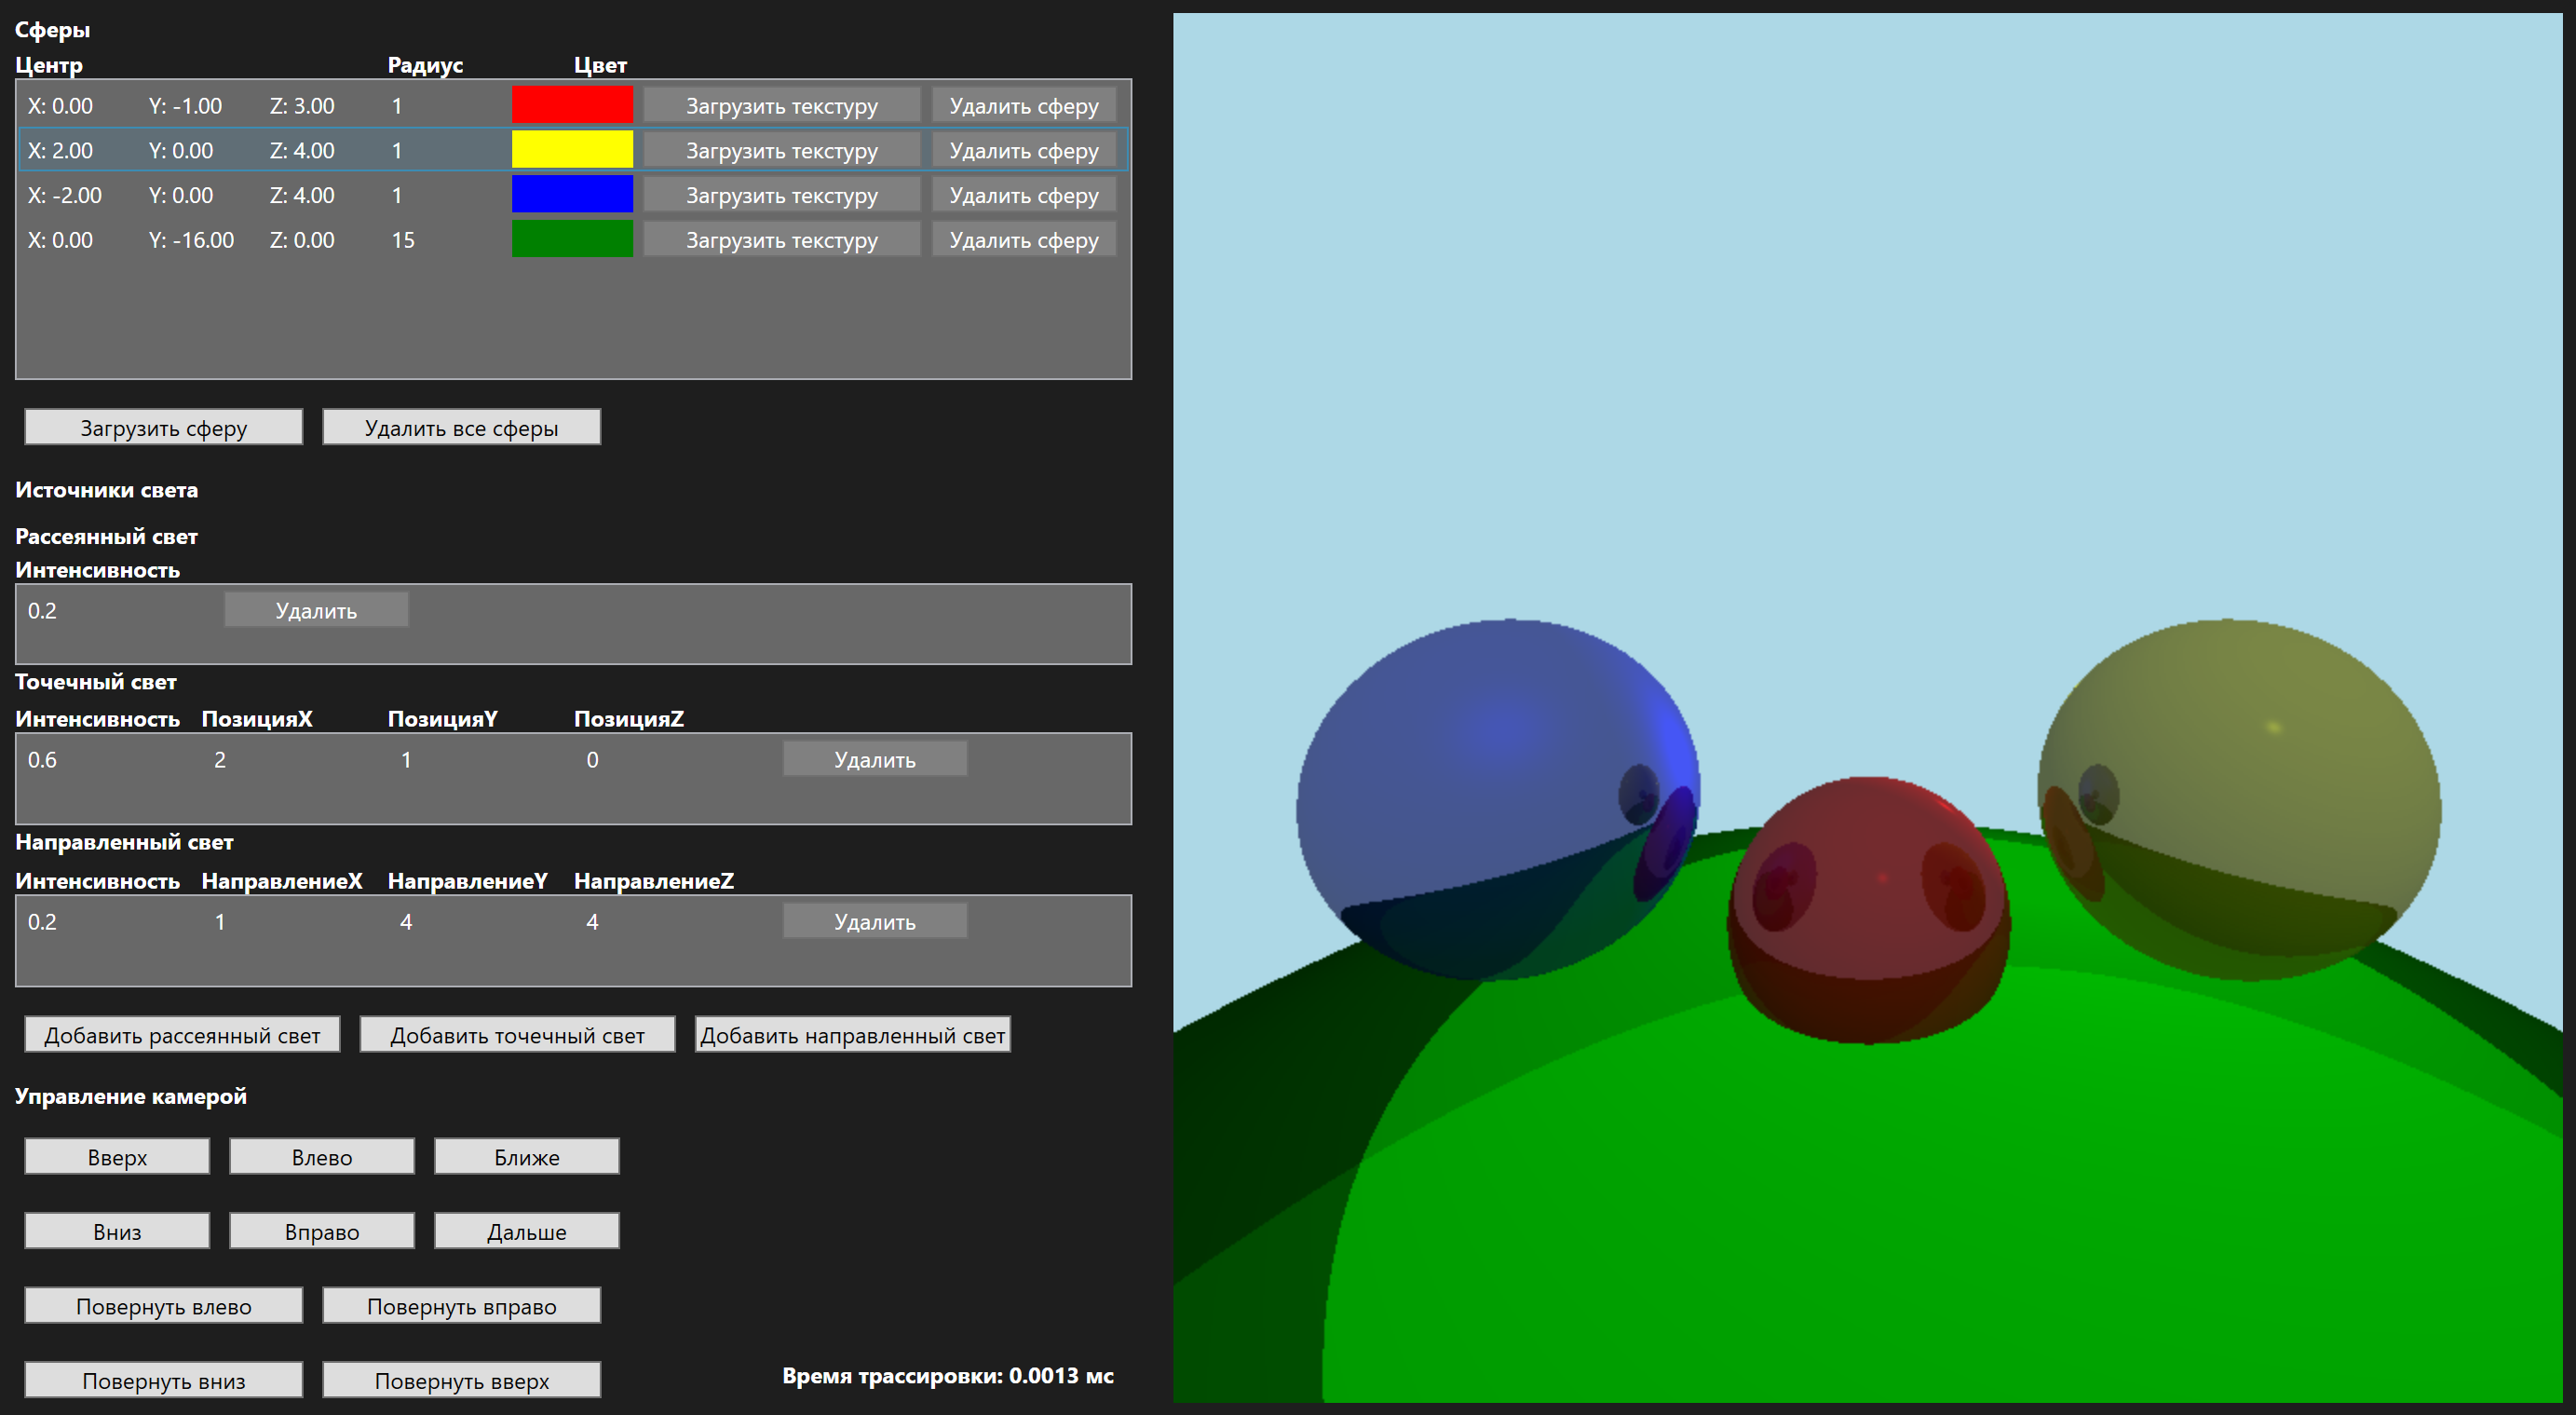
\includegraphics[width=0.85\linewidth]{include/3-2.png}
		\captionof{figure}{Интерфейс ПО}
		\label{img:3-2}
	\end{tabular}
\end{table}

В левой части экрана расположены списки всех сфер и источников света на сцене, а так же различные кнопки: добавления и удаления сфер, наложения текстур на сферу, перемещения и вращения камеры, добавления и удаления света. В нижней части расположено поле, в котором отображается время выполнения трассировки сцены.

\section*{Вывод}
В этом разделе были выбраны средства реализации программы и составлена диаграмма классов, представлена реализация алгоритмов и пользовательский интерфейс.
